% !TEX program = xelatex
% English version: AISS 2026 Challenge
% Build: tools/build_paper.sh (xelatex x2 + bibtex)
% Discipline: no experimental number is hand-copied into the text;
%   all figures are injected via numbers.tex macros. Re-run
%   tools/gen_paper_numbers.py after the batch freeze to update the paper.
\documentclass[10pt,twocolumn]{article}
\usepackage{geometry}
\geometry{a4paper,top=2.2cm,bottom=2.4cm,left=1.8cm,right=1.8cm,columnsep=0.75cm}
% 仅作者姓名含中文字符，需 xeCJK；正文全英文不受影响
\usepackage{xeCJK}
\setCJKmainfont{Songti SC}
\usepackage{graphicx}
\usepackage{booktabs}
\usepackage{amsmath}
\usepackage[numbers,sort&compress]{natbib}
\usepackage{xcolor}
\usepackage{caption}
\usepackage{hyperref}
\hypersetup{colorlinks=true,linkcolor=black,citecolor=blue!50!black,urlcolor=blue!50!black}
\captionsetup{font=small,labelfont=bf}
% 章节标题不做连字符断词（避免 "Sim-ulation" 这类断法）
\usepackage{titlesec}
\titleformat{\section}{\normalfont\Large\bfseries\raggedright}{\thesection}{1em}{}
\titleformat{\subsection}{\normalfont\large\bfseries\raggedright}{\thesubsection}{1em}{}
\setlength{\bibsep}{2pt}
\renewcommand{\bibfont}{\small}

\usepackage{etoolbox}
% 自动生成（tools/gen_paper_numbers.py），勿手改
% 生成日期 2026-09-13
\newcommand{\ValidRuns}{11}
\newcommand{\TargetRuns}{12}
\newcommand{\DraftBadge}{}
\newcommand{\DraftBadgeEn}{}
\newcommand{\IsoIvNone}{29.4}
\newcommand{\LonIvNone}{37.7}
\newcommand{\IsoPostNone}{27.2}
\newcommand{\IsoRebNone}{-2.2}
\newcommand{\NNone}{3}
\newcommand{\IsoIvCasework}{7.9}
\newcommand{\LonIvCasework}{29.4}
\newcommand{\IsoPostCasework}{27.5}
\newcommand{\IsoRebCasework}{+19.6}
\newcommand{\NCasework}{3}
\newcommand{\IsoIvTimebank}{24.7}
\newcommand{\LonIvTimebank}{36.3}
\newcommand{\IsoPostTimebank}{25.6}
\newcommand{\IsoRebTimebank}{+0.8}
\newcommand{\NTimebank}{3}
\newcommand{\IsoIvPlatform}{23.5}
\newcommand{\LonIvPlatform}{35.4}
\newcommand{\IsoPostPlatform}{27.5}
\newcommand{\IsoRebPlatform}{+4.0}
\newcommand{\NPlatform}{2}
\newcommand{\CaseworkIvReduction}{73\%}
\newcommand{\PairIvCasework}{-21.5}
\newcommand{\PairIvCaseworkN}{3}
\newcommand{\PairRebCasework}{+21.8}
\newcommand{\PairRebCaseworkN}{3}
\newcommand{\PairIvTimebank}{-4.7}
\newcommand{\PairIvTimebankN}{3}
\newcommand{\PairRebTimebank}{+3.1}
\newcommand{\PairRebTimebankN}{3}
\newcommand{\PairIvPlatform}{-5.6}
\newcommand{\PairIvPlatformN}{2}
\newcommand{\PairRebPlatform}{+4.8}
\newcommand{\PairRebPlatformN}{2}
\newcommand{\DelayCostCasework}{+0.15}
\newcommand{\DelayCostTimebank}{+0.18}
\newcommand{\DelayCostPlatform}{+0.00}
\newcommand{\TimingSeeds}{20}
\newcommand{\RulesBaselineOverall}{15.0}
\newcommand{\RulesRebCwLo}{+7.9}
\newcommand{\RulesRebCwHi}{+9.5}
\newcommand{\RulesRebTb}{+2.1}
\newcommand{\CaseCwRun}{casework\_s1}
\newcommand{\CaseCwAgent}{18}
\newcommand{\CaseCwLonWd}{0.19}
\newcommand{\CaseCwLonEnd}{0.50}
\newcommand{\CaseCwTiesWd}{7}
\newcommand{\CaseCwTiesEnd}{6}
\newcommand{\LoopIters}{5}
\newcommand{\LoopBestDesc}{casework start=4 dur=12}
\newcommand{\LoopBestScore}{7.70}
\newcommand{\FocIvNone}{56.9}
\newcommand{\FocPostNone}{51.8}
\newcommand{\RulIvNone}{17.7}
\newcommand{\RulPostNone}{16.7}
\newcommand{\FocShareNone}{58\%}
\newcommand{\FocLonIvNone}{0.56}
\newcommand{\FocLonPostNone}{0.58}
\newcommand{\RulLonIvNone}{0.30}
\newcommand{\RulLonPostNone}{0.33}
\newcommand{\FocIvCw}{13.0}
\newcommand{\FocPostCw}{63.0}
\newcommand{\RulIvCw}{5.8}
\newcommand{\RulPostCw}{12.3}
\newcommand{\FocShareCw}{49\%}
\newcommand{\FocLonIvCw}{0.42}
\newcommand{\FocLonPostCw}{0.52}
\newcommand{\RulLonIvCw}{0.24}
\newcommand{\RulLonPostCw}{0.29}
\newcommand{\PFocIvCw}{-44.0}
\newcommand{\PFocRebCw}{+55.1}
\newcommand{\PRulIvCw}{-11.9}
\newcommand{\PRulRebCw}{+7.5}
\newcommand{\FocIvTb}{45.8}
\newcommand{\FocPostTb}{52.8}
\newcommand{\RulIvTb}{15.7}
\newcommand{\RulPostTb}{13.9}
\newcommand{\FocShareTb}{56\%}
\newcommand{\FocLonIvTb}{0.54}
\newcommand{\FocLonPostTb}{0.57}
\newcommand{\RulLonIvTb}{0.29}
\newcommand{\RulLonPostTb}{0.31}
\newcommand{\PFocIvTb}{-11.1}
\newcommand{\PFocRebTb}{+12.0}
\newcommand{\PRulIvTb}{-2.0}
\newcommand{\PRulRebTb}{-0.8}
\newcommand{\FocIvPf}{43.1}
\newcommand{\FocPostPf}{56.9}
\newcommand{\RulIvPf}{15.2}
\newcommand{\RulPostPf}{14.9}
\newcommand{\FocSharePf}{55\%}
\newcommand{\FocLonIvPf}{0.52}
\newcommand{\FocLonPostPf}{0.53}
\newcommand{\RulLonIvPf}{0.28}
\newcommand{\RulLonPostPf}{0.29}
\newcommand{\PFocIvPf}{-11.1}
\newcommand{\PFocRebPf}{+13.9}
\newcommand{\PRulIvPf}{-3.3}
\newcommand{\PRulRebPf}{+0.9}
\newcommand{\CostTotal}{1056}
\newcommand{\CostValid}{529}
\newcommand{\CostWasted}{409}
\newcommand{\CostModelCompare}{118}
\newcommand{\WasteShare}{44\%}
\newcommand{\TotalCalls}{45,901}

\graphicspath{{../figures/}}

\title{\textbf{A Scientific Discipline for LLM Social Simulation:\\ Layered Generative Agents Applied to Social Support Interventions for Older Adults Living Alone}}
\author{Dongshuai Hui (惠栋帅) \quad Caihou Wang (王才厚) \quad Mingren Lei (雷明仁)\\ \small AISS 2026 Challenge Submission}
\date{}

\begin{document}
\twocolumn[
\maketitle
\vspace{-2em}
\ifdefempty{\DraftBadgeEn}{}{\begin{center}\fbox{\parbox{0.92\textwidth}{\small\DraftBadgeEn}}\end{center}}
\vspace{0.5em}
\begin{minipage}{\textwidth}
\begin{center}\textbf{Abstract}\end{center}
\small
Multi-agent LLM social simulation faces a threefold challenge: are the data fabricated, are the conclusions reproducible, and are the ``findings'' merely echoes of the environment's rules? Using social support interventions for older adults living alone as a case study, we propose and demonstrate a \textbf{scientific discipline} for LLM social simulation: preregistered hypotheses and validity gates, anchoring to real survey data, archiving and root-cause classification of failed runs, cost accounting that includes sunk costs, and an item-by-item \textbf{``prescribed vs.\ emergent'' ledger}. The simulation, built on AgentSociety2, embeds six LLM-driven focal elders in a 20-person rules-layer support network (1 step = 1 month, 24 months) and compares professional casework, timebank mutual aid, and digital-platform volunteer matching, implemented in months 7--18 and then withdrawn for six months. Results (\ValidRuns/\TargetRuns\ valid runs): casework yields the lowest in-window isolation rate (\IsoIvCasework\% vs.\ a \IsoIvNone\% baseline) and rebounds by \IsoRebCasework pp after withdrawal; the timebank rebounds by \IsoRebTimebank pp. We state plainly that this sustainability divergence is the expected pattern \emph{reproduced} under explicitly encoded mechanism assumptions (immediate contact on intervention, a pairing-persistence probability), not an emergent discovery; a layer decomposition shows that \FocShareNone\ of the macro isolation rate comes from the LLM layer, and that the timebank's ``no rebound'' is mainly a rules-layer contribution, while the LLM layer still rebounds by \PFocRebTb pp. The genuinely emergent results lie in the behavioural layer: the three interventions leave distinguishable help-seeking signatures, with casework generating the most requests at the lowest success rate; and a cross-model check finds that gpt-6-astra is more inclined to ``do nothing'' when no intervention is present, while visits from an external actor pull decisions out of it---a finding with general implications for validity-gate design in LLM social simulation. All results reproduce from the released scripts in a single command.\par\vspace{0.4em}
\noindent\textbf{Keywords}: generative agents; social support networks; older adults living alone; social work interventions; timebank; multi-agent simulation
\end{minipage}
\vspace{1.2em}
]

\section{Introduction}
Loneliness and social isolation among Chinese adults aged 65+ who live alone are problems of considerable scale: in the CLHLS 2008/09 wave, 52\% of older adults living alone reported feeling lonely, nearly twice the share among those living with others (29.5\%)\citep{wei2022living} (cited for the scale of the problem; our calibration uses the 2021 wave living-alone subsample under an ``often/always'' criterion, so the two figures differ in wave and definition and are not directly comparable). Social-work practice has developed several intervention routes---professional casework, community mutual aid (timebanks), and digital-platform volunteering---but two key questions remain stubbornly out of reach of the empirical literature:

\textbf{(1) What happens after the intervention is withdrawn?} RCTs and quasi-experiments almost always measure outcomes during or at the end of the programme\citep{lu2024timebank}; the post-withdrawal counterfactual trajectory is unobservable in the real world: one cannot both deliver and withhold an intervention from the same cohort.

\textbf{(2) When is entry most worthwhile?} Waiting lists and budget constraints make the start date a genuine policy variable, yet the marginal cost of timing has never been systematically quantified.

Generative-agent simulation\citep{park2023generative} offers a new instrument: LLM-driven agents produce reasoned behavioural decisions in a controlled environment, and identical random seeds allow ``parallel worlds'' to be replayed. Multi-agent LLM simulation nevertheless faces a threefold challenge---are the data fabricated, are the conclusions reproducible, and are the ``findings'' merely echoes of the environment's rules? This paper makes three contributions:

\begin{enumerate}
  \item \textbf{A transferable scientific discipline}: preregistered hypotheses and validity gates, dimension-by-dimension anchoring to real survey data, archiving and root-cause classification of failed runs (infrastructure-type vs.\ behavioural-type), true-cost accounting including sunk costs, and a \textbf{``prescribed vs.\ emergent'' ledger} that marks, item by item, which results follow directly from the environment's rules and which are new information produced by the simulation (Table~\ref{tab:prescribed}).
  \item \textbf{A layered hybrid architecture and its decomposition}: an LLM focal layer (six elders) embedded in a rules layer (20-person network) whose zero-API-cost dynamics support large-sample scans; we further decompose the isolation-rate trajectories of the two layers from the traces, quantifying the weight of the LLM layer in the macro outcome and the behavioural differences between layers (Table~\ref{tab:layers}).
  \item \textbf{Two behavioural-layer findings about LLM agents as subjects of social simulation}: (i) the three interventions leave distinguishable help-seeking signatures on focal elders, with casework producing the most requests at the lowest success rate; (ii) a cross-model check shows gpt-6-astra is more inclined to ``do nothing'' without an intervention, while visits from an external actor pull decisions out of it, suggesting that validity gates must be designed jointly with model characteristics.
\end{enumerate}
Beyond these, the post-withdrawal sustainability divergence (H4) and the delay cost of entry timing are reported as \emph{expected patterns reproduced under explicit mechanism assumptions, together with their sensitivity ranges}---not as emergent findings.

\section{Related Work and Theoretical Basis}
\textbf{Social support theory and the convoy model.} The convoy model\citep{kahn1980convoys} views an older person's social ties as layered convoys moving through the life course: the inner circle (spouse, children) is stable but eroded by widowhood and health shocks, while the outer circle (neighbours, friends) is more fluid. Our relationship ledger operationalises this structure directly: every tie has a strength, a type, and a most-recent-contact month, and decays when contact lapses.

\textbf{The empirical shape of tie decay.} Burt's cross-study fits show that decay rates are non-constant and follow a power function---``older ties are more stable''\citep{burt2000decay}; tie termination among older adults has also been measured directly\citep{kleinikkink1999broken}. In Section~\ref{sec:honest} we measure our model's survival curves against Burt's yardstick and report the structural deviation candidly.

\textbf{Effect-size evidence for loneliness interventions.} The meta-analysis by Masi et al.\ provides an effect-size yardstick for four intervention classes (social-cognitive interventions largest, $d=-0.598$)\citep{masi2011meta}; the subtype breakdown of Hoang et al.\ shows technology-based interventions with CIs crossing zero and multi-component interventions significant in community settings\citep{hoang2022interventions}. Two casework RCTs (older adults living alone\citep{ristolainen2020effects}; community-dwelling frail elders\citep{taube2018case}) point in the same direction with conservative ITT estimates. Quasi-experimental timebank evidence indicates effects lasting at least to programme end with no crowding-out\citep{lu2024timebank}. These effect sizes and directions supply both the parameter basis and the outcome benchmark for our three interventions.

\textbf{Generative-agent simulation.} Park et al.\ established the paradigm of LLM agents producing believable social behaviour\citep{park2023generative}. This paper differs in its policy-comparison purpose: a preregistered experimental design, calibration to real survey data, and systematic validity checking.

\section{Method: Layered Hybrid Simulation}
\subsection{Overall architecture}
The simulation is built on the AgentSociety2 framework (Ray parallelism, full tracing, replayable decisions). Twenty older adults living alone form a support network; six of them are \textbf{LLM focal elders} (PersonAgent, model gpt-5.6-sol) who, each month, run a multi-round tool loop to perceive the environment, retrieve memory, act, and articulate a natural-language rationale. The remaining fourteen residents and all network dynamics (tie decay, monthly events, intervention mechanics) are driven by the \textbf{rules layer} and consume no LLM calls. The focal layer supplies mechanistic and narrative evidence; the rules layer preserves the integrity of the network structure and supports zero-cost large-sample sensitivity scans. Measured call density is roughly 13.8 calls per focal elder per month. \textbf{The two layers generate contact differently}: rules-layer elders automatically receive contact each month according to their child-contact frequency and extroversion; focal elders receive contact only through their own tool actions (calling family, visiting neighbours, seeking help, attending activities) and through visits by intervention actors---a month in which the LLM takes no action is recorded as a month without contact. This difference is the direct cause of the threefold gap in isolation levels between layers reported in Section~\ref{sec:layers}, and it means the focal-layer isolation rate measures both ``is the elder isolated'' and ``did the LLM act''.

\subsection{Environment and the relationship ledger}
The environment module (ElderSupportEnv) maintains a relationship ledger for every elder: tie type (child / neighbour / friend / volunteer / social worker), strength $s\in[0,1]$, monthly contact frequency, and most recent contact month. A tie with no contact in a given month decays as $s \leftarrow s\times(1-\delta)$ (baseline $\delta=0.06$; sensitivity scan 0.15/0.25) and is deleted at $s<0.05$. Monthly events include health shocks, widowhood (triggering a loneliness jump calibrated to the CHARLS +27pp risk difference and CLHLS widowhood dynamics\citep{yang2021widowhood}), and child visits. Loneliness $\ell\in[0,1]$ is driven by tie activation and events; $\ell\ge0.6$ counts as ``lonely'' (mapping to CLHLS item b38 ``often/always'', baseline target about 15\%).

\subsection{The three interventions}\label{sec:interventions}
\begin{itemize}
  \item \textbf{casework --- professional case management}: after risk-ranked assessment, social workers visit high-risk elders and reconnect them with family; top-down and precise, but constrained by caseload. Parameters draw on Masi's social-cognitive effect class\citep{masi2011meta} and the two casework RCTs\citep{ristolainen2020effects,taube2018case}; the coverage cap equals the number of workers $\times$ caseload.
  \item \textbf{timebank --- time-bank mutual aid}: younger-old healthy elders are paired with high-risk elders and exchange services for credits under automatic rules; the pairings are real interpersonal ties and persist after withdrawal with probability post\_persist (midpoint 0.5, scanned 0.3--0.7). Parameters draw on the Hong Kong timebank quasi-experiment\citep{lu2024timebank}; no literature point estimate exists for post-withdrawal persistence, so it is treated as a scan.
  \item \textbf{platform --- digital volunteer matching}: responsive, broad-coverage, rotating volunteers, shallow ties. Its effect is set weakest of the three, following meta-analytic evidence that technology-based interventions have CIs crossing zero\citep{hoang2022interventions}.
\end{itemize}

\subsection{Data calibration}
The profile generator is anchored dimension by dimension to real surveys: sex (63.8\% female), self-rated health, a five-level loneliness baseline, number of surviving children, and the share of children who visit regularly (78.7\%) come from the CLHLS 2021 living-alone subsample; child proximity comes from CHARLS 2015; longitudinal anchors (three-year loneliness onset 27.2\% among those living alone, persistence 53.3\%, widowhood shock +27pp) come from Harmonized CHARLS 2011--2018. Outcome-definition mappings and known biases (reweighting for CLHLS oversampling of the oldest-old, unweighted panel attrition, etc.) are documented in the appendix and repository. The only output-side external-validity check available so far is this: the simulated three-year incidence gradient of new loneliness matches in direction and magnitude the living-alone vs.\ co-residing incidence gap reported by Wei et al.\ (34.0\% vs.\ 22.3\%)\citep{wei2022living}, and since that difference is not significant after covariate adjustment it serves only as descriptive corroboration. The tie-decay shape, by contrast, explicitly fails to match the Burt fit (Section~\ref{sec:honest}). Stated honestly: \textbf{calibration alignment currently holds on the input side; the model's dynamics have not yet passed any strict external-validity test}---the most important gap for future work.

\subsection{Preregistration and validity gates}\label{sec:prereg}
Hypotheses (H1--H4), primary and secondary outcomes, seeds, and validity criteria were written into script headers before the formal batch was launched:
\textbf{primary outcome} isolation\_rate (monthly isolation rate, defined as the share of elders with no emotional-support contact in the month); \textbf{secondary outcome} avg\_loneliness; deep\_isolation\_rate enters sensitivity analyses only, and avg\_active\_ties is descriptive only. \textbf{Validity gates}: a run must complete 24 months, have non-empty decision records, focal-elder silence rate $\le$10\%, and LLM call error rate $\le$5\%; any violation renders the run invalid and triggers a full rerun, with invalid runs archived rather than deleted. With $n=3$ seeds we perform no significance tests and claim no stable ranking; H4 is a within-run paired contrast (post-withdrawal $-$ intervention window) and is flagged as exploratory.

\textbf{Nature and limits of the primary outcome.} isolation\_rate is a monthly snapshot of ``was there any emotional contact this month''. Any presence-based service delivered monthly (casework triggers one emotional contact with probability 0.8 for each covered elder each month) drives it to zero by definition, so within the intervention window the indicator mainly measures ``is the service present''; the step changes at months 7 and 19 in Fig.~\ref{fig:traj} arise from this. Loneliness $\ell$ is a continuous quantity with homeostatic dynamics (each month it moves halfway toward a set point determined by contact volume, tie count, health, and personality) and is closer to a genuine outcome. The preregistration lists it as secondary; we do not alter that status, but we \textbf{report the two side by side} and, when interpreting effect sizes, treat loneliness as the outcome and the isolation rate as the ``presence'' indicator.

\section{Experimental Design}
Four conditions (none / casework / timebank / platform) $\times$ 3 seeds $\times$ 24 months, targeting \TargetRuns\ valid runs, of which \ValidRuns\ were frozen: platform seed~2 was ruled invalid because the focal elders' silence rate reached 11.3\% (17/150 agent-months), above the 10\% gate (LLM error rate 0; silence clustered in gateway-timeout steps, i.e.\ an infrastructure failure), and could not be rerun before the deadline, so the platform arm is reported with $n=\NPlatform$; the intervention window spans months 7--18, with post-withdrawal observation in months 19--24. Hypotheses:
\textbf{H1} all three interventions lower the isolation rate during the window, with casework lowering it most;
\textbf{H2} loneliness improves in the same direction during the window;
\textbf{H3} the three interventions leave distinguishable behavioural signatures (help-seeking routes, pairing, volunteer matching);
\textbf{H4} (exploratory) casework rebounds more than the timebank after withdrawal---structural mutual aid is more sustainable.

\section{Main Results (LLM Behavioural Layer)}\label{sec:results}
\DraftBadgeEn

\begin{table}[t]
\centering\small
\caption{Primary outcome by window (isolation rate, \%; condition means). Rebound $=$ post-withdrawal $-$ intervention window, pp.}
\label{tab:main}
\begin{tabular}{lcccc}
\toprule
Condition & $n$ & Interv. & Post & Rebound \\
\midrule
none      & \NNone     & \IsoIvNone     & \IsoPostNone     & \IsoRebNone \\
casework  & \NCasework & \textbf{\IsoIvCasework} & \IsoPostCasework & \textbf{\IsoRebCasework} \\
timebank  & \NTimebank & \IsoIvTimebank & \IsoPostTimebank & \IsoRebTimebank \\
platform  & \NPlatform & \IsoIvPlatform & \IsoPostPlatform & \IsoRebPlatform \\
\bottomrule
\end{tabular}
\end{table}

\begin{figure*}[t]
\centering
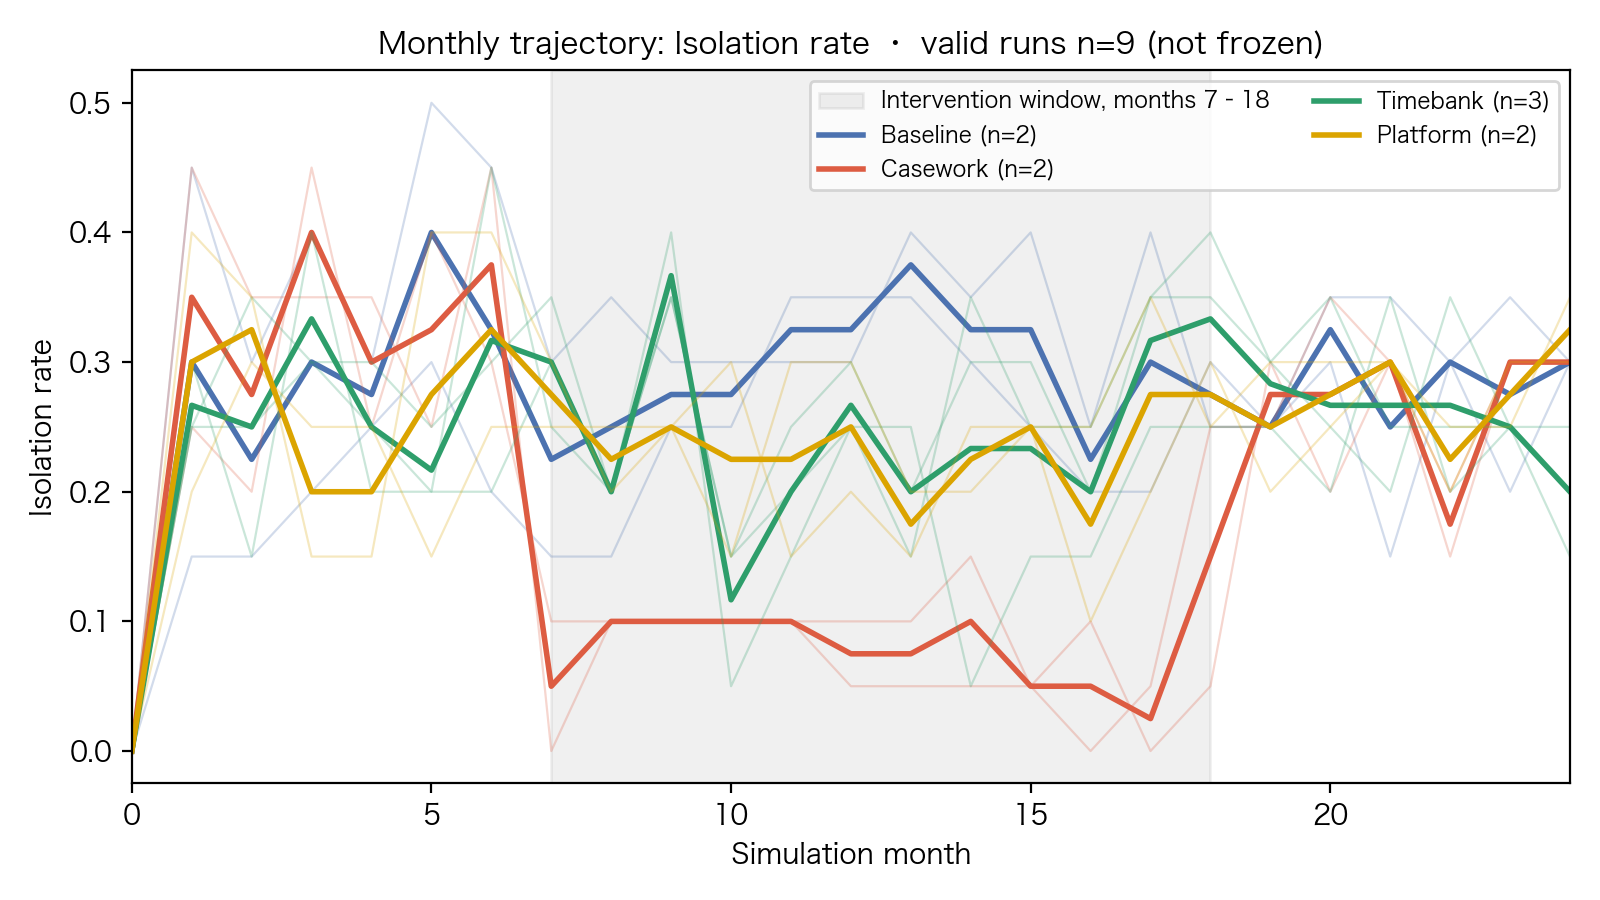
\includegraphics[width=0.95\textwidth]{fig1_trajectory_isolation_en.png}
\caption{Monthly isolation-rate trajectories (thick lines: condition means; thin lines: individual seeds; shading: intervention window, months 7--18). The casework arm shows step changes at months 7 and 19, corresponding to the entry and exit of a presence-based service (see Section~\ref{sec:prereg} on the nature of the primary outcome).}
\label{fig:traj}
\end{figure*}

\subsection{During the intervention: casework leads}
During the window, casework yields an isolation rate of \IsoIvCasework\%, a relative reduction of \CaseworkIvReduction\ against the \IsoIvNone\% baseline; the same-seed paired difference is \PairIvCasework pp (paired $n=$\PairIvCaseworkN). The timebank (\IsoIvTimebank\%) and platform (\IsoIvPlatform\%) improve outcomes only modestly. Loneliness (reported alongside) moves in the same direction but with a much smaller magnitude: casework \LonIvCasework\% vs.\ baseline \LonIvNone\% (a relative reduction of about 22\%, against \CaseworkIvReduction\ for the isolation rate)---the gap between the two indicators is itself evidence that the isolation rate mainly measures service presence. The direction is consistent with the Masi meta-analysis, in which cognitively oriented interventions show the largest effects\citep{masi2011meta}, supporting H1/H2.

\subsection{H4: a sustainability divergence reproduced under explicit mechanism assumptions}
After withdrawal, the casework isolation rate rebounds by \IsoRebCasework pp (same-seed paired difference \PairRebCasework pp), all but erasing the in-window advantage; the timebank rebounds by \IsoRebTimebank pp (Figs.~\ref{fig:traj} and~\ref{fig:paired}). A 20-seed rules-layer scan shows the same shape (casework rebound \RulesRebCwLo\ to \RulesRebCwHi pp, timebank \RulesRebTb pp).

\textbf{This must be stated plainly: it is not an emergent finding.} Both mechanisms are written into the environment. Casework's emotional contact is triggered directly by the social worker's monthly visit and disappears on withdrawal; timebank pairings continue to interact after withdrawal with probability post\_persist (midpoint 0.5), and the code comment explicitly labels this persistence probability ``the key mechanism assumption for H4''. LLM focal elders and rules-layer elders inhabit the same environment and share the same indicator definition, so the rules layer and the LLM layer are \emph{not} two independent lines of evidence; the ``cross-layer corroboration'' wording of an earlier draft is withdrawn here. The accurate statement of H4 is: \textbf{under explicitly encoded mechanism assumptions, the simulation reproduces the expected sustainability divergence and provides its sensitivity range} (direction unchanged across post\_persist 0.3--0.7; caseload 4--12 does not alter the rebound). Its value lies in turning the practice intuition ``dependency-type support vanishes on exit, reciprocal ties partly persist'' into a parameterised, refutable model---not in proving it true. The most informative supplementary experiment would set post\_persist to zero and check whether the divergence disappears; we have not run it and list it as future work.

\subsection{Layer decomposition: the weight of the LLM layer in the macro outcome}\label{sec:layers}
Table~\ref{tab:layers} decomposes the window means of the six focal elders and the fourteen rules-layer elders from the replays. Three observations. (1) \textbf{Focal elders' baseline isolation rate is about three times that of rules-layer elders} (none: \FocIvNone\% vs.\ \RulIvNone\%), a consequence of the contact-generation difference described in Section 3.1---an LLM elder that does not act has no contact. (2) \textbf{The LLM layer dominates the macro effect}: focal elders are 30\% of the population but contribute \FocShareNone\ of the baseline isolation rate, and casework's paired effect on the focal layer (in-window \PFocIvCw pp, rebound \PFocRebCw pp) is three to seven times its effect on the rules layer (\PRulIvCw pp, \PRulRebCw pp). ``Generative-agent simulation'' is therefore not decorative---but it also means the headline results are highly sensitive to LLM behavioural traits, including silence. (3) \textbf{The timebank's ``no rebound'' is mainly a rules-layer contribution}: the rules-layer paired rebound is \PRulRebTb pp (post\_persist at work), whereas the LLM layer rebounds by \PFocRebTb pp, comparable to the platform arm (\PFocRebPf pp) and much smaller only than casework (\PFocRebCw pp). What the LLM layer supports is thus ``casework rebounds far more than the other two'', not ``the timebank barely rebounds''. Loneliness moves in the same direction in both layers, with gentler magnitudes.

\begin{table}[t]
\centering\small
\caption{Layer decomposition (window means; isolation in \%, loneliness 0--1). Focal = six LLM elders, Rules = fourteen rules-layer elders; paired difference = condition $-$ none under the same seed.}
\label{tab:layers}
\resizebox{\columnwidth}{!}{%
\begin{tabular}{lcccccc}
\toprule
 & \multicolumn{2}{c}{Focal isolation} & \multicolumn{2}{c}{Rules isolation} & \multicolumn{2}{c}{Loneliness focal/rules} \\
Condition & Window & Post & Window & Post & Window & Post \\
\midrule
none     & \FocIvNone & \FocPostNone & \RulIvNone & \RulPostNone & \FocLonIvNone/\RulLonIvNone & \FocLonPostNone/\RulLonPostNone \\
casework & \FocIvCw & \FocPostCw & \RulIvCw & \RulPostCw & \FocLonIvCw/\RulLonIvCw & \FocLonPostCw/\RulLonPostCw \\
timebank & \FocIvTb & \FocPostTb & \RulIvTb & \RulPostTb & \FocLonIvTb/\RulLonIvTb & \FocLonPostTb/\RulLonPostTb \\
platform & \FocIvPf & \FocPostPf & \RulIvPf & \RulPostPf & \FocLonIvPf/\RulLonIvPf & \FocLonPostPf/\RulLonPostPf \\
\midrule
\multicolumn{7}{l}{Paired difference vs.\ none (pp): in-window / rebound} \\
casework & \multicolumn{2}{c}{\PFocIvCw\ / \PFocRebCw} & \multicolumn{2}{c}{\PRulIvCw\ / \PRulRebCw} & & \\
timebank & \multicolumn{2}{c}{\PFocIvTb\ / \PFocRebTb} & \multicolumn{2}{c}{\PRulIvTb\ / \PRulRebTb} & & \\
platform & \multicolumn{2}{c}{\PFocIvPf\ / \PFocRebPf} & \multicolumn{2}{c}{\PRulIvPf\ / \PRulRebPf} & & \\
\bottomrule
\end{tabular}}
\end{table}

\begin{figure}[t]
\centering
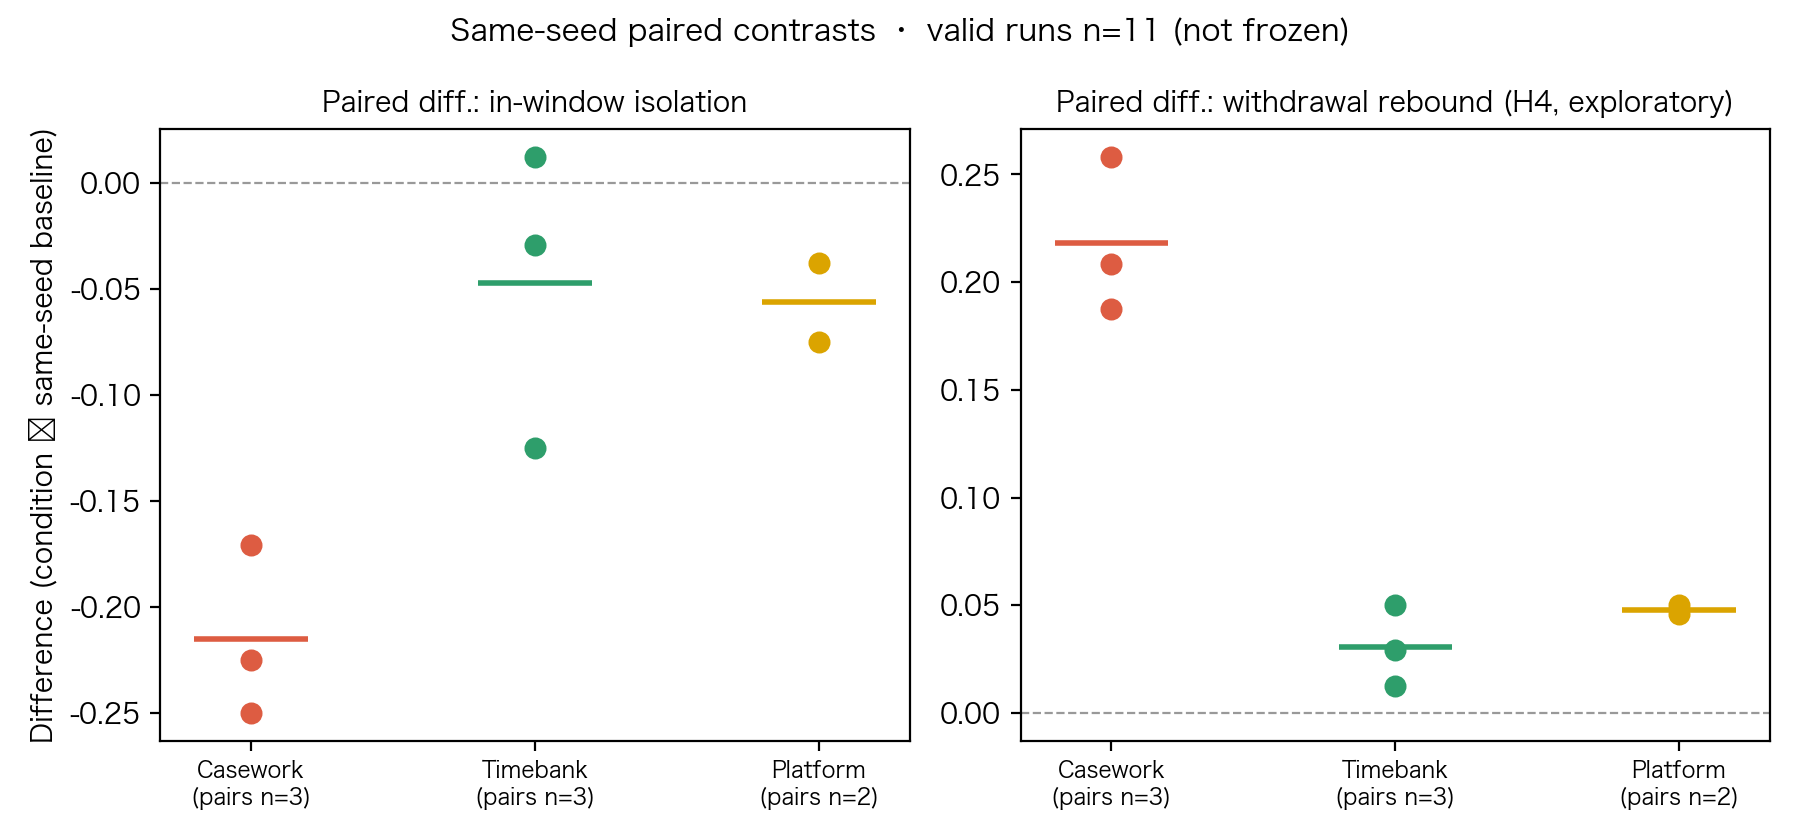
\includegraphics[width=\columnwidth]{fig4_paired_rebound_en.png}
\caption{Same-seed paired contrasts (left: in-window effect; right: post-withdrawal rebound, exploratory).}
\label{fig:paired}
\end{figure}

\subsection{Behavioural signatures and mechanistic corroboration (H3)}
The three interventions leave clearly distinguishable signatures in the focal elders' behaviour logs\footnote{Help-request statistics over the \ValidRuns\ valid runs (\texttt{tests/behavior\_signature.json}): none, 3 runs, 249 requests / 183 successful (73.5\%, 83.0 per run); timebank 247/185 (74.9\%, 82.3); casework 412/271 (65.8\%, 137.3); platform, 2 runs, 159/94 (59.1\%, 79.5).}: the timebank arm has the highest help-success rate of any condition (mutual-aid pairing at work); the casework arm generates by far the most help requests (proactive social-worker outreach) but a below-average success rate; the baseline and timebank arms request at similar volumes, while the platform arm has the fewest requests per run and the lowest success rate. Casework's ``most requests, lowest success rate'' deserves elaboration: the social worker is the most reachable tie in the ledger, LLM elders issue help requests more often while a worker is present (including requests to the worker), and after withdrawal they keep requesting from a target that no longer responds, so failed requests accumulate. This is a behavioural-layer result not prescribed by any rule, consistent with practice descriptions of ``dependency-type support''---but, like the rest of this section, a descriptive observation over three seeds. The so-called \textbf{``tie-count paradox''} (active-tie counts remain high after withdrawal while the isolation rate rebounds) must be characterised for what it is: social-worker ties decay slowly in the ledger ($\delta=0.06$) and still count as active for months after exit, whereas the isolation rate only asks whether contact occurred this month. The paradox is a direct consequence of the indicator definitions, not new mechanistic evidence; its narrative value is to remind us that ``a tie exists'' and ``a tie functions'' are two different quantities.

An individual trajectory makes the paradox concrete (preregistered case-selection rule: among valid casework runs, the focal elder who received a social-worker visit before withdrawal and shows the largest post-withdrawal loneliness rebound; exploratory evidence). Elder \CaseCwAgent\ in \CaseCwRun\ stood at loneliness \CaseCwLonWd\ with \CaseCwTiesWd\ active ties at the point of withdrawal (month 18); by month 24 the network had shrunk by a single tie (\CaseCwTiesEnd), yet loneliness had climbed to \CaseCwLonEnd---the network was nearly intact; what vanished was the social-worker node that activated it. No counterpart timebank case from a valid run exists (the only run with an explicit pairing record failed the silence gate, so its case is excluded from evidence), which we state plainly. The practice implication: casework should build in referral toward reciprocal networks and an exit plan.

\subsection{Reporting a cross-layer discrepancy candidly}
The in-window ranking is not fully consistent across layers: the rules layer puts timebank above platform, while the LLM layer puts platform slightly above timebank (platform has only \NPlatform\ valid seeds; the difference cannot be separated from seed noise). It is mechanistically explicable: the LLM layer's platform intervention introduces new volunteer ties and raises active-tie counts. We report this as ``a cross-layer difference and its explanation'' rather than concealing it---exposing exactly such inconsistencies is where the layered design earns its keep.

\section{Mechanism Layer: Timing, Dosage, and an Autonomous Loop}\label{sec:mechanism}
\subsection{The delay cost of entry timing}
A preregistered rules-layer scan (start month $\{3,5,7,9,12\}\times$ duration $\{6,12,18\}\times$ 3 conditions, \TimingSeeds\ seeds; baseline full-horizon isolation rate \RulesBaselineOverall\%) yields three findings:
\begin{enumerate}
  \item \textbf{Interventions act immediately}: within the window, the isolation rate barely varies with start month---the entire cost of delay comes from unprotected waiting months, not from ``missing a critical window'';
  \item \textbf{A directional estimate of delay cost}: each month of postponement raises the two-year mean isolation rate by about \DelayCostCasework pp (casework) / \DelayCostTimebank pp (timebank), about 3.6 pp over 24 months against a \RulesBaselineOverall\% baseline; the platform's total effect is weak, so it is timing-insensitive (\DelayCostPlatform pp). The magnitude is fixed entirely by the rule property ``interventions act immediately'' (Table~\ref{tab:prescribed}) and is offered only as a directional estimate under the rules-layer mechanism;
  \item \textbf{Rebound is dose-independent}: extending casework from 6 to 12 months does not soften the post-withdrawal rebound (\RulesRebCwLo\ to \RulesRebCwHi pp)---the rebound of dependency-type support is a property of the mechanism, not a symptom of underdosing.
\end{enumerate}
Disclosures: a later start implies a shorter post-withdrawal observation window (a confound), and the 18-month duration has no post-window at all; rules-layer absolute levels are not compared with the LLM batch---only direction and magnitude are used. An LLM-behavioural-layer timing contrast across prevention / early-warning / crisis stages has \emph{not} been run; it is future work, and we do not write plans as results.

\subsection{An autonomous harness loop}
We demonstrate an automated research loop under preregistration constraints: an LLM designer proposes candidate configurations round by round within a preregistered search space (condition $\times$ start month 3--12 $\times$ duration 6--12, objective: minimise full-horizon isolation rate, resource cap duration $\le$12), a deterministic rules-layer evaluator executes them, and all \LoopIters\ rounds are logged to disk. The loop converges to \LoopBestDesc\ (full-horizon isolation rate \LoopBestScore\%), within one seed standard deviation of the grid optimum---\textbf{the loop works as a procedure, and we report candidly that it rediscovered the grid's plateau without surpassing it}. The guardrails (LLM proposes only; evaluation is deterministic; space and round count preregistered; every round logged) ensure the demonstration introduces no selective reporting. In addition, the per-run automated analysis--reflection mechanism (analyze.py) currently implements ``detect and flag'': any change to the experimental configuration requires human review, preventing mid-experiment design drift.

\section{Scientific Checks and Honest Bias Reporting}\label{sec:honest}
\subsection{Calibration alignment and emergent validity}
Input distributions are aligned with the survey data dimension by dimension (Section 3.4). Run-level dynamics are cross-checked against the literature: the simulated widowhood shock matches the direction of CLHLS widowhood--loneliness dynamics (OR 3.09 in the first years of widowhood)\citep{yang2021widowhood}. Table~\ref{tab:prescribed} distinguishes, item by item, which of this paper's results follow directly from the environment's rules and which are new information from the simulation. The table is our direct answer to the objection that LLM simulation merely echoes its rules: at the level of macro outcomes, most of the main patterns are prescribed; the emergent content is concentrated in the LLM behavioural layer.

\begin{table}[t]
\centering\small
\caption{Prescribed vs.\ emergent: the nature of each result in this paper.}
\label{tab:prescribed}
\resizebox{\columnwidth}{!}{%
\begin{tabular}{@{}p{0.50\columnwidth}p{0.19\columnwidth}p{0.40\columnwidth}@{}}
\toprule
Result & Nature & Source \\
\midrule
Immediate response of isolation to intervention (step at month 7) & prescribed & indicator definition $+$ monthly visit triggers contact \\
Casework rebound after withdrawal & prescribed & no visit, no contact \\
Timebank persistence after withdrawal (rules layer) & prescribed & post\_persist param.\ (0.5; scan 0.3--0.7) \\
Linear accrual of delay cost by month & prescribed & direct consequence of immediate onset \\
Tie-count paradox (ties remain, activation gone) & prescribed & decay slower than the monthly snapshot \\
Threefold isolation gap between layers & semi-prescribed & different contact generation (Sec.~3.1); magnitude not preset \\
Timebank LLM layer still rebounds \PFocRebTb pp & emergent & LLM elders do not act on pairings spontaneously \\
Distinguishable help-seeking signatures & emergent & focal-elder tool-call distribution \\
Casework: most requests, lowest success & emergent & focal-elder behaviour logs \\
gpt-6-astra: quieter without intervention, pulled by visits & emergent & cross-model comparison \\
Behavioural silence concentrated in the window & emergent & failed-run diagnosis \\
\bottomrule
\end{tabular}}
\end{table}

\subsection{Structural limits of tie decay}
Measuring our model's tie-survival curves against Burt's yardstick (rules layer, 50 persons $\times$ 48 months) reveals two \textbf{mechanism-level limits}: (1) tie loss is markedly slower than in the literature (4-year survival 78.8\% vs.\ 38.3\% under Burt's fit); (2) there is a survival floor of about 46\%---children with fixed contact schedules and high-frequency neighbours refresh their contact timestamps monthly, never enter the decay branch, and thus no value of $\delta$ can reproduce the sustained decline of Burt's power function. Accordingly we \textbf{do not treat tie-loss rate as a calibration target}, only as a sensitivity dimension. One correction attaches to the Burt citation: the paper's ``2.63-year half-life for ties outside the family'' is an arithmetic slip (a constant term left unsubtracted); recomputed from the paper's own equation it is 1.63 years\citep{burt2000decay}. The deep-isolation measure is truncated by the survival floor and therefore enters sensitivity analyses only.

\subsection{Modelling choices handled as scans}
Three independent literature searches (the third via a multi-source aggregator covering CrossRef/OpenAlex/arXiv) concurred: no authoritative source supports $\delta=0.06$ or caseload $=8$---search results that conjured ``perfectly matching'' numbers (the project encountered one fabricated reference and one fabricated statistic in its first search round) were all rejected and archived. These two parameters are therefore treated as \textbf{modelling choices}: $\delta$ is scanned over 0.06/0.15/0.25 (scan points chosen from the measured survival curves); caseload in this model effectively controls intervention coverage of high-risk elders (4/8/12 mapping to 40\%/80\%/100\%), a different unit from real-world client rosters---measured average rosters in New York City home-bound elder case management run around 75 clients per worker and are considered overloaded\citep{pardasani2018caseload}. The Chinese industry standard specifies staffing ratios but no caseload clause\citep{mzt064}, and NASW explicitly declines to set a uniform caseload standard\citep{nasw2013}, so the scan is expressed in coverage terms. Scan conclusions: $\delta$ shifts overall levels but does not reorder the interventions; caseload is monotone within the window and converges after withdrawal---coverage affects the in-place effect, not sustainability.

\subsection{Root-cause diagnosis of failed runs}
Every run failing the validity gates (Section~\ref{sec:prereg}) was archived and diagnosed, revealing two failure modes: (1) \textbf{infrastructure failures}---LLM gateway error storms blacking out whole months of decisions (errors visibly clustered in the trace), handled by rerunning with a higher retry count (an infrastructure parameter, not a protocol change); (2) \textbf{behavioural failures}---the LLM reasons normally but initiates no environmental action, concentrated inside the intervention window and consistent with the casework dependency mechanism. The latter has no infrastructure fix; such runs are rerun under the preregistered gate, and if the pattern recurs the run is excluded per the rules while the tension is reported in the limitations (the gate may conflate ``silent malfunction'' with ``legitimate dependent inaction''), with an additional sensitivity analysis that retains the run---the gate itself is not altered.

\subsection{Model and inference-setting disclosure}
The formal batch uses a single model (gpt-5.6-sol) with uniform sampling settings; reasoning-effort level was not recorded by the run script and is disclosed as ``not recorded'', to be supplemented with a small-sample contrast. Cross-model robustness (a gpt-6-astra contrast batch: the none and casework runs at seed~1) is treated as a sensitivity check outside the main results; see Section~\ref{sec:robust}.

\subsection{Cross-model sensitivity check}\label{sec:robust}
We swap the focal elders' driving model for gpt-6-astra, keeping every other setting (profiles, seed, intervention parameters, horizon) identical to the seed-1 main-batch runs, rerun the none and casework conditions, and ask whether the casework$-$none in-window isolation gap and the direction of the post-withdrawal rebound agree with the main model. Single seed, two conditions: a descriptive directional check with no significance claim. Results and silence rates are in Table~\ref{tab:robust}.

\textbf{Same direction.} Under both models casework relative to none shows ``lower isolation in-window $+$ larger rebound after withdrawal'': the paired gap is $-17.1$~pp in-window and $+18.8$~pp in rebound for the main model, versus $-25.0$~pp and $+25.0$~pp for gpt-6-astra, whose two arms return to the identical post-withdrawal level (30.0\% each), i.e.\ the casework effect vanishes completely once the worker leaves---consistent with the ``injected node'' reading above.

\textbf{Behavioural silence is a model trait, not a random fault.} Two independent gpt-6-astra runs of the none arm (same seed) produced silence rates of 10.7\% (16/150 agent-months) and 11.3\% (17/150), both crossing the 10\% validity gate and ruled invalid by rule; LLM error rates were 0.17\% and 0, and the silent months were spread across several elders rather than clustered in gateway-timeout steps, unlike the infrastructure-type failure of platform seed~2. All 11 sol runs in the main batch stay at $\le 10\%$ (none seed~1: 4.0\%), while the same astra model's casework arm is silent only 2.0\% of the time---a persistently visiting external actor appears to ``pull'' decisions out of astra elders, whereas left alone this model more often issues no action at all. We report this as a robustness finding in its own right: (i) the gate was calibrated on the main model and may be systematically strict for more ``taciturn'' models, which the limitations section acknowledges; (ii) the astra none-arm isolation rates in the table are directional only and enter no headline result; (iii) a third rerun was deliberately declined to avoid ``run until it passes'' selective reporting.

\textbf{General implications for validity-gate design in LLM social simulation.} The finding reaches beyond this case. (a) ``Doing nothing'' in an LLM agent may be a fault or may be the model's default behavioural tendency, and that tendency varies across models and with whether an active external actor is present in the environment; a gate calibrated on a single model therefore biases cross-model comparisons toward the more ``action-prone'' model. (b) The presence of an external actor pulls decisions out of LLM agents, so silence rates are naturally asymmetric between intervention and control arms; a silence-rate gate is stricter on the control arm and can inflate estimated intervention effects. (c) A practical remedy is to express the gate as a relative quantity (the silence-rate difference between intervention and control arms) or to preregister a per-model baseline silence rate. We recommend that future LLM social-simulation work report ``baseline silence rate without intervention'' as a mandatory model-selection statistic.

\begin{table}[t]
\centering\small
\caption{Cross-model sensitivity check (seed~1, single run). Isolation rates are window means (\%); rebound $=$ post $-$ in-window (pp); silence rate is the share of focal-elder agent-months with no decision (gate 10\%).}
\label{tab:robust}
\resizebox{\columnwidth}{!}{%
\begin{tabular}{llcccc}
\toprule
Model & Condition & Silence & In-window & Post & Rebound \\
\midrule
gpt-5.6-sol & none     & 4.0\% & 25.8 & 25.0 & $-0.8$ \\
            & casework & 8.7\% & 8.8  & 26.7 & $+17.9$ \\
gpt-6-astra & none     & 11.3\%$^\dagger$ & 29.6 & 30.0 & $+0.4$ \\
            & casework & 2.0\% & 4.6  & 30.0 & $+25.4$ \\
\midrule
\multicolumn{2}{l}{Paired casework$-$none: sol}   & & $-17.1$ & $+1.7$ & $+18.8$ \\
\multicolumn{2}{l}{Paired casework$-$none: astra} & & $-25.0$ & $0.0$ & $+25.0$ \\
\bottomrule
\end{tabular}}

\smallskip
{\footnotesize $^\dagger$ Exceeds the 10\% gate and is ruled invalid; the first attempt (10.7\%, 16/150) crossed it as well. Behavioural metrics are directional only.}
\end{table}

\section{True Cost Accounting}
Cost reporting for multi-agent LLM experiments must include runs eliminated by quality gates. This project accumulated \TotalCalls\ LLM calls (measured from traces, archived invalid runs included), with an estimated total cost of \$\CostTotal: \$\CostValid\ on valid main-batch runs, \$\CostWasted\ sunk on invalid ones (a \WasteShare\ share of the main batch), plus \$\CostModelCompare\ for the cross-model contrast arms (Section~\ref{sec:robust}). Token usage is a documented assumption (traces do not record per-call usage) and unit prices follow public pricing; the full accounting basis is released with the data files. Here the layered design pays off concretely: the rules-layer scans (\TimingSeeds\ seeds $\times$ 45 configurations) and the harness loop cost zero API dollars; running the same scans through the LLM layer would exceed the main batch's cost by an order of magnitude.

\section{Discussion and Policy Implications}
\textbf{(1) Waiting time is a modellable intervention design variable.} Under the rules-layer mechanism, interventions act immediately and delay cost accrues linearly by the month (about \DelayCostCasework pp/month). This is a directional estimate only: it presupposes that an intervention produces contact as soon as it is in place, and real start-up lags and coverage ramp-ups would change the magnitude.

\textbf{(2) Casework needs a built-in exit plan.} Strongest in-window effect and largest post-withdrawal rebound are two faces of one mechanism: the social worker is an injected active node. The rebound does not soften with dosage, suggesting that exit design (gradual tapering, referral into reciprocal networks) should be a standard component of casework rather than an option---consistent with the ``ties remain, activation is gone'' narrative (whose nature is discussed in Section~\ref{sec:results}).

\textbf{(3) The sustainability of structural mutual aid is a hypothesis to test, not a conclusion.} The timebank's post-withdrawal persistence is prescribed in the rules layer by post\_persist and did not arise spontaneously in the LLM layer (focal elders rebound by \PFocRebTb pp). ``Casework to open, timebank to sustain'' should therefore be posed as a follow-up hypothesis and tested against a post\_persist $=0$ control to see whether it depends on that parameter.

\textbf{(4) Timing talk is pointless for weak interventions.} Platform-type interventions have weak total effects and are timing-insensitive---secure intensity first, then optimise timing.

All of the above are model-mechanism conclusions intended to generate testable policy hypotheses; \textbf{we claim no causal effects in real populations}.

\section{Limitations and Ethics}
\textbf{Limitations.} (1) $n=3$ seeds ($n=\NPlatform$ for the platform arm) support only descriptive contrasts and directional judgements, not significance or stable rankings; (2) the tie-decay mechanism has a 46\% survival floor and is slower than the empirical shape in the literature; (3) the behavioural validity of LLM focal elders depends on the model itself, and behavioural silence is hard to separate from a real elder's ``legitimate inaction'', and the 10\% silence gate was calibrated on the main model gpt-5.6-sol and may be systematically strict for models more inclined to inaction (gpt-6-astra's none arm: 10.7--11.3\% in two attempts; see Section~\ref{sec:robust}); (4) calibration sources differ in definitions (survey waves; living-alone subsample vs.\ full sample); (5) the post-withdrawal observation window is only six months; (7) the primary outcome isolation\_rate is a monthly contact snapshot hit directly by presence-based services, so effect sizes should be read from loneliness; (8) more than half of the macro outcome is contributed by six LLM elders, making the headline results highly sensitive to LLM behavioural traits; (6) the Ristolainen RCT's subgroup effect suffers from non-comparable baselines\citep{ristolainen2020effects}, so casework parameters lean primarily on the Masi meta-analysis.

\textbf{Ethics.} All agents are simulated entities; no real individuals are involved. Survey data enter only as aggregate distributions from public microdata. The LLM-generated ``elders' rationales'' are mechanistic probes, not real elders' voices, and the paper avoids quoting them anthropomorphically. Because simulation conclusions could be misused as direct grounds for resource allocation, we repeatedly stress their hypothesis-generating character.

\section{Conclusion}
The main product of this paper is a scientific discipline for LLM social simulation, demonstrated end to end on social support interventions for older adults living alone: preregistration with validity gates, real-data anchoring with honest deviation reporting, root-cause classification of failures, cost transparency including sunk costs, a guardrailed autonomous experimentation loop, and an item-by-item ``prescribed vs.\ emergent'' ledger. Within the case, casework's in-window lead and the post-withdrawal sustainability divergence are expected patterns reproduced under explicit mechanism assumptions; the layer decomposition shows that the macro outcome is dominated by the LLM layer and that the timebank's persistence comes mainly from the rules layer. The new information genuinely produced by the simulation lies in the behavioural layer: distinguishable help-seeking signatures, casework's high-request/low-success profile, and gpt-6-astra's greater silence without intervention and responsiveness to visits---the last with general implications for validity-gate design across the field. We draw these boundaries sharply so that follow-up work (a post\_persist $=0$ control, per-model baseline silence calibration, an LLM-layer timing contrast) has clear targets. Every number updates automatically from the scripts; we invite reproduction per the appendix.

\bibliographystyle{unsrtnat}
\bibliography{refs}

\appendix
\section{Reproducibility Checklist}\label{app:repro}
\begin{itemize}
  \raggedright % 清单多为不可断行的等宽路径，两端对齐会把行内空白拉得过大
  \item \textbf{Code and data}: AgentSociety2 repository \texttt{examples/v2/elder\_support/}; environment module \texttt{custom/envs/elder\_support\_env.py}.
  \item \textbf{Formal batch}: \texttt{run\_batch.sh 24 1 2 3} (automatic checkpoint resumption; validity gates and archiving built in).
  \item \textbf{Analysis and figures}: \texttt{tools/compare\_conditions.py} $\rightarrow$ \texttt{comparison.json}; \texttt{tools/make\_figures.py} (each figure ships with a same-name CSV); \texttt{tools/gen\_paper\_numbers.py} (the sole source of every number in this paper).
  \item \textbf{Mechanism scans and loop}: \texttt{tests/scan\_timing.py}, \texttt{tools/harness\_loop.py} (preregistered headers + per-round JSONL audit logs).
  \item \textbf{Cost and diagnosis}: \texttt{tools/cost\_report.py}, \texttt{tests/silence\_diagnosis.json}.
  \item \textbf{Calibration documents}: \texttt{data\_pipeline/out/calibration\_targets.md}, \texttt{references\_verified.md} (including rejected entries and verification methods).
  \item \textbf{Live dashboard}: \url{https://agentsociety.shangdian.me} (batch progress, conclusion cards, mechanism evidence, cost and failure diagnosis).
\end{itemize}

\section{Validity-Gate Adjudication Rules}
A run is valid if and only if: the DONE flag exists; monthly metrics for months 0--24 are complete; decision records are non-empty; the six focal elders' combined silence rate is $\le$10\% (strictly greater than 0.10 fails); and the LLM call error rate is $\le$5\%. Invalid runs are archived under timestamped directories (\texttt{*.invalid-<timestamp>}) with all traces and decision logs preserved for diagnosis---never deleted.

\end{document}
